\documentclass[journal]{./IEEE/IEEEtran}
\usepackage{cite,graphicx}


\newcommand{\SPTITLE}{Tourist Sentiment Analysis in the Philippines: A Comparative Study Using NLP Before and After COVID-19}
\newcommand{\ADVISEE}{Rita Isabel P. Colina}
\newcommand{\ADVISER}{Dr. Maria Art Antonette D. Clariño}

\newcommand{\BSCS}{Bachelor of Science in Computer Science}
\newcommand{\ICS}{Institute of Computer Science}
\newcommand{\UPLB}{University of the Philippines Los Ba\~{n}os}
\newcommand{\REMARK}{\thanks{Presented to the Faculty of the \ICS, \UPLB\
                             in partial fulfillment of the requirements
                             for the Degree of \BSCS}}
        
\markboth{CMSC 190 Special Problem, \ICS}{}
\title{\SPTITLE}
\author{\ADVISEE~and~\ADVISER%
\REMARK}
% \pubid{\copyright~2006~ICS \UPLB}

%%%%%%%%%%%%%%%%%%%%%%%%%%%%%%%%%%%%%%%%%%%%%%%%%%%%%%%%%%%%%%%%%%%%%%%%%%

\begin{document}

% TITLE
\maketitle

% % ABSTRACT
% \begin{abstract}
% The abstract should be \textit{informational}. Typically a single paragraph
% of about fifty to two hundred workds, the abstract allows your readers to judge
% whether or not the article is of relevance to them. It should therefore be
% a concise summary of the aims, scope, and conclusions of your work. There
% is no space for unnecessary texts; an abstract should be kept to as few words
% as possible while remaining reasonably informative. Irrelevancies, such as
% minor details or a \textit{description} of the structure of the paper, are 
% inappropriate, as are acronyms, abbreviations, and mathematics. Sentences such
% as ``we review relevant literature" should be omitted.\cite{Zobel97}
% \end{abstract}

% % INDEX TERMS
% \begin{keywords}
% key, words, separated, by, comma
% \end{keywords}

% INTRODUCTION
\section{Introduction}

\subsection{Background of the Study}
The tourism industry is among the sectors that have been greatly affected by the COVID-19 pandemic.\cite{one:ugur2020impacts}
Preventive measures to help stop the spread of the virus such as lockdowns, curfews, and travel restrictions, were implemented worldwide. 
These actions, while vital for public health, resulted in the closure of borders, airports, hotels, 
transportation, and other forms of mass gatherings. These negatively impacted the tourism sector of the Philippines, 
and consequently, its gross domestic product (GDP)

In 2019, the Philippines tourism industry contributed 12.7\%  of the nations GDP. It provided 5.71 million jobs 
in the same year. When the period of travel restrictions in most countries started in the first quarter of 2020, 
tourism-related businesses opted to temporarily stop offering their products and services, either due to restrictions or to low demands, resulting in a significant crash in the tourism and economic sectors of the country. \cite{two:pwc-tourism-covid19}


\subsection{Research Problem}
A survey conducted by PWC \cite{two:pwc-tourism-covid19} revealed that 78\% of decision-makers in the tourism services sector 
(i.e., travel agencies, bookings, tours, operations, etc.) need up to 5 million Philippine Pesos (PHP) 
in additional funding to normalize their operations, particularly to facilitate the rebuilding and 
refinancing of their businesses. While governmental financial assistance is underway, the study 
highlights the importance of accelerating the digital transformation of tourism services and enhancing 
operational digitalization as critical strategies to speed up the recovery of the country’s tourism 
industry. Moreover, the surge in global social media usage post-pandemic, notably on platforms like Twitter and 
Facebook, presents new avenues for crisis communication, information dissemination, and sentiment analysis 
within the tourism sector. The emergence of social networking services (SNS) has facilitated widespread expression
of opinions, offering researchers unique opportunities to analyze user-generated data, including sentiments, 
intentions to travel, and perspectives on COVID-19 concerns\cite{one:ugur2020impacts} such as vaccination, public health, and governance during lockdown 
periods. This convergence of challenges and opportunities underlines the need for comprehensive research to understand and 
address the evolving dynamics within the tourism industry in response to the COVID-19 crisis and the digital 
transformation reshaping the sector. 

\subsection{Scope and Delimitation}
The scope of this study encompasses the application of NLP techniques for sentiment analysis specifically focused on tweets related to tourism in the Philippines. The study aims to analyze sentiments expressed in tweets before and after the COVID-19 pandemic to understand the evolving perceptions and attitudes of local travelers towards Philippine tourism destinations. The analysis will be conducted using a Recurrent Neural Network (RNN) model trained on a dataset of tweets from November 2018 to November 2019 and January 2023 to January 2024, geotagged within the Philippines and within a 200,000 kilometer radius.

The study acknowledges the limitations inherent in the size and composition of the dataset. The analysis will be based on the available tweets collected during the specified time frame and geographical scope. 

Sentiment analysis  will be conducted using an RNN model trained on the collected dataset. While RNNs are effective for sequence modeling tasks, the performance of the model may be influenced by factors such as data quality, feature representation, and model architecture.

The interpretation of sentiment analysis results will be based on the insights derived from the RNN model and the analytical techniques employed. Human interpretations may be subjective and influenced by other factors such as contextual understanding, domain expertise, and qualitative analysis of the sentiment patterns observed. 


\subsection{Significance of the Study}
This study aims to address a critical gap in existing literature concerning tourist sentiments before and after the COVID-19 pandemic lockdown. While prior studies have predominantly focused on the early stages of the pandemic, there remains a lack of research that systematically compares tourist perceptions over time. By undertaking this comparative analysis, the study aims to contribute valuable insights into the evolving attitudes and preferences of travelers towards the Philippines as a destination amidst the pandemic’s enduring impact. This research holds significant implications for the recovery and sustainability of the Philippines’ tourism sector, offering actionable insights into the factors shaping tourist behavior and destination choices. Moreover, the study aims to apply Natural Language Processing (NLP) techniques in tourism sentiment analysis.

\subsection{Objectives of the Study}
The study aims to use Artificial Intelligence (AI) to compare and analyze Twitter posts regarding tourism in the Philippines between the pre-pandemic and post-pandemic lockdown periods. Natural language processing and sentiment analysis techniques will be applied in order to successfully polarize these posts. The specific objectives of this research are as follows:

\begin{enumerate}
  \item\label{item:this} To automatically categorize Tweets based on positive, negative, or neutral sentiments regarding travel to the Philippines,
  \item\label{item:that} To identify tourist sentiment towards the Philippines before and after the COVID-19 lockdown,
  \item\label{item:these} To identify the key factors that affect Philippine tourism after the COVID-19 lockdown,
  \item \label{item:those} To identify the impact of the risks of COVID-19 on tourism sentiments
  \end{enumerate}

% RRL
\section{Review of Related Literature}
\subsection*{Tourism Efforts in the Philippines}
In 2012, the Department of Tourism (DOT) launched the It’s More Fun in the Philippines tourism branding campaign to motivate and attract travelers and tourists worldwide to visit the Philippines. The rebrand was done to replace the former campaign WOW! Philippines and to match the worldwide tourism marketing standards and be competitive at the global level. In the same year, foreign arrivals already increased by 11.9\%. Since then, the hashtag \#itsmorefuninthephilippines was widely used for travel and tourism-related posts in various social networking sites.\cite{three:rappler-philippines-tourism} The campaign continued to progress from 2013 to 2019, with sustained engagement and positive feedback from both domestic and international audiences. However, the onset of the COVID-19 pandemic in 2020 brought unprecedented challenges to the tourism sector, resulting in a sharp decline in tourist arrivals and a significant impact on the country’s GDP.

During the pandemic era spanning from 2020 to 2022, the tourism sector in the Philippines experienced a great downturn, mirroring the broader economic challenges reflected in GDP statistics. The imposition of travel restrictions and mobility limitations, coupled with economic uncertainties, posed formidable obstacles to the sector’s recovery efforts.\cite{four:statista-philippines-tourism} 

In June 2023, DOT released Love the Philippines as part of a strategic rebranding initiative to relaunch the country’s tourism campaign and support its recovery efforts. However, the campaign’s release was immediately met with online criticism, primarily due to the incorporation of stock videos of tourist attractions from other countries including Brazil, Switzerland, Thailand, Indonesia, and the United Arab Emirates. As a result, DOT terminated its contract with DDB Philippines, the marketing agency responsible for the campaign’s publication materials. DOT, however, reaffirmed its commitment to the Love the Philippines slogan.\cite{five:mb-enhanced-tourism-slogan} 

The public response to the launch of the Love the Philippines campaign highlights the significance of social media engagement in the tourism sector. Feedback and transparency in government projects like this iare instrumental to the aid for the country’s recovery from the negative effects of the pandemic lockdown. 

\subsection*{Natural Language Processing Applications on Tourism and Hospitality}

A number of studies have focused on applying machine learning techniques in the tourism sector. A study by Alvarez-Carmona et al.,\cite{six:alvarez} reviewed 227 journal articles that applied NLP in tourism research. Its main objective was to know how NLP was used in the tourism industry and to comprehend the current status of NLP research in hospitality and tourism. The researchers were able to create a novel taxonomy of studies that employ NLP in tourism research by applying NLP themselves using the PRISMA methodology. The study was able to classify the studies into five (5) major categories: sentiment analysis, destination branding, question-answering, NLP for assisting in tourism, and miscellaneous. The study was also able to identify the most important processes in using NLP, which are preprocessing, representation methods, machine learning algorithms, and performance metrics. They were able to conclude that hotel reviews and data from TripAdvisor were the preferred data source, and that deep learning techniques are most successful when utilizing NLP, but the amount of data and the involvement of different languages were common hindrances to the studies. 

A study by Menchavez et al., \cite{seven:menchavez} in 2015 was able to automatically classify Tweets as tourism or non-tourism related, as well as apply sentiment analysis on them. The researchers applied feature extraction, bag of words, and classification using various machine learning techniques such as the Naïve Bayes classifier, logistic regression, and support vector machines (SVM). The study also compared the performance of these AI models and concluded that SVMs yielded the highest accuracy and F-scores, and Naïve Bayes with n-grams also yielded great results. A recommendation from this study was to focus on specific cities and/or provinces rather than gathering data from the whole Philippines in order to address more specific problems and concerns. 

Another similar study by Sontayasara et al., \cite{eight:Sontayasara_2021jdr} applied sentiment analysis on Tweets about Bangkok tourism during the COVID-19 pandemic. The researchers used the Twitter API to collect tweets, then manually annotated a part of their dataset in order to train their AI model (SVM). The results concluded that the most used words in the Tweets were “food”, “city”, and “temple”. The sentiment of the majority of people wanting to visit Bangkok for the food and the tourist attractions (i.e. temples) were evident. 

\subsection*{Sentiment Analysis After COVID-19}

A recent study by Ugur et al., \cite{one:ugur2020impacts} analyzed text from TripAdvisor documents, web pages, and comments regarding trips and bookings during the early stages of the pandemic. Text mining, word frequency, and word clouds were used to apply sentiment analysis on a statistical approach. Their study concluded that cancellation of trips were mentioned most at a rate of 40.81\% amongst all of the cases they reviewed, and “travel insurance” was the second most frequently repeated phrase after “coronavirus”. They were also able to conclude that the tourism sector is very easily affected by global crises, and that it takes extra time for travelers to return to their old mobility even after the crisis has ended. 

Another study using statistical sentiment analysis aimed to discuss the underlying socioeconomic factors for polarized sentiments in the United States of America (USA). Rahman, et al., \cite{nine:RAHMAN2021e06200} analyzed Twitter data using a binary logit model to explore sentiments on reopening the economy after the COVID-19 lockdown. The researchers concluded that family households, people with low education attainment, people in the labor force, low-income people, and people with higher house rent were more interested in reopening the economy than people with higher income. The model they used correctly classified 56.18\% of the sentiments, and a Pearson chi-squared test indicated that the model has high goodness-of-fit. They were able to indicate and suggest to policymakers where to allocate resources and which policy options can be undertaken to improve the socioeconomic situations of the people and mitigate the impacts of the pandemic in the current situation, as well as in the future. 

--

The aforementioned studies offer insights into various aspects of tourism research, marketing, crisis communication, and sentiment analysis. However, there remains a lack of research that systematically compares local tourist sentiments regarding the Philippines over time, specifically before and after the COVID-19 pandemic lockdown. This study aims to bridge these gaps by utilizing NLP techniques and examining the evolving perceptions, attitudes, and sentiments of local travelers towards the Philippines as a destination amid the pandemic’s disruptive impact. Furthermore, the review highlights the potential of NLP applications in tourism and hospitality research, as demonstrated by studies that have successfully employed machine learning techniques to analyze tourist-related tweets and sentiment dynamics in other contexts. Through this, this study aims to uncover nuanced patterns in tourist sentiments, offering valuable insights for policymakers, decision makers, industry stakeholders, and marketers seeking to enhance tourism recovery efforts in the post-pandemic era.



% MATERIALS AND METHODS
\section{Materials and Methods}

\begin{figure}
  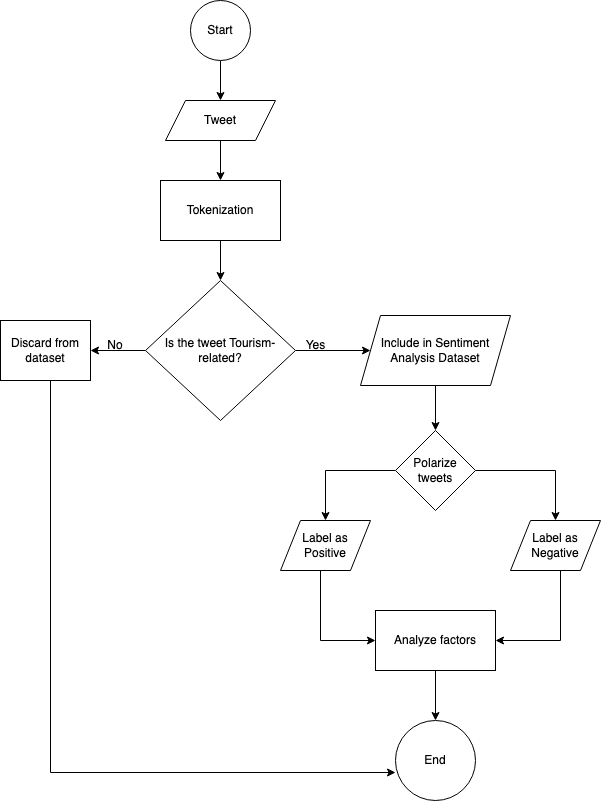
\includegraphics[width=\linewidth]{images/methods.drawio.png}
  \caption{The general process of the methodology of the study}
  \label{fig:methodology}
\end{figure}

Figure 1 shows the general process or flow of the experiment being proposed. Each tweet from the dataset is taken as an input and will be tokenized. It will then be categorized as tourism or non tourism-related. If it is tourism-related, then it will be included in the dataset for sentiment analysis. During this process, each tweet will be further categorized into positive, negative, or neutral sentiments. The features extracted and factors considered will be observed in order to answer the research objectives of this study. Further details about the methodology will be discussed in the subsections below. 

\subsection{Dataset}
A total of 10,012 tweets were scraped from twitter.com for analysis, dated November 2018 to November 2019, and December 2022 to December 2023. Only Tweets geotagged from the Philippines and within a 200,000 kilometer radius were considered for inclusion in the dataset. The keywords used for the search were “Philippines”, “travel”, “tour”, “vacation”, “visit”, “more fun in the philippines”, “\#itsmorefuninthephilippines”, and “\#philippinestravel”, with “Philippines” as a required keyword. 


\subsection{Preprocessing}
\subsubsection{Tokenization}
Links will be removed from each tweet. They will then undergo tokenization, lemmatization, and will be converted to lowercase. If hashtags are present in the tweet, then it will be converted into separate words. 
\subsubsection{Identification of Tourism/Non tourism-related Tweets}
The tweets will be represented by a vector containing all unique words used in all of the tweets. A dictionary will be created for each tweet and the frequency of each word will be counted. The dictionaries will be used to classify each tweet as tourism or non tourism-related. 

	20\% (2,002 tweets) of the dataset will be used to train the Bag-of-Words model, and the rest will be automatically classified using the Naïve Bayes classifier. This will be implemented using Python with NLTK. N-grams and weights will be used and adjusted if necessary for better accuracy, precision, recall, and f-scores. 

	The Naïve Bayes classifier is a supervised machine learning algorithm that models the distribution of inputs for a given class. It assumes that the features (words) of the input data are conditionally independent given the class (i.e. each tweet belonging to either the Tourism or Nontourism class). It will calculate the probability of a tweet belonging to each class based on word frequency. \cite{ten:analyticsvidhya-naive-bayes}

	This process will be done to automate the preprocessing step for identifying tweets that will be included in the sentiment analysis portion of the experiment.

\subsection{Sentiment Analysis}
Recurrent Neural Networks (RNN) will be used to polarize sentiments and analyze its factors. 

The RNN architecture can handle sequential data by maintaining an internal state or memory, which can be applied to words in sentences and paragraphs. It is a discriminative AI model, wherein differences between the positive and negative sentiments are taken into account in order to perform classification. \cite{eleven:geeksforgeeks-rnn-text-classification} 

The Naïve Bayes classifier was also considered for the sentiment analysis part of this study. However, since one of the researcher’s objectives is to find out underlying factors and reasonings behind tourist sentiments, the RNN architecture is implied to be more appropriate. By using its attention mechanisms, the researchers may be able to infer causes of the sentiment outcomes from which words or phrases contribute most to the sentiment analysis decisions. The Naïve Bayes’ assumption of independence for each feature makes it less suitable than the RNN because of the lack of consideration of context for each tweet.

The RNN will be implemented using Python with deep learning libraries such as KerasNLP and Tensorflow. 

\subsection{Performance Metrics}
\subsubsection{Naïve Bayes Classifier}
To determine the accuracy, precision, f-scores, and recall performance of the Naïve Bayes classifier for classifying tourism and non tourism-related tweets, 10-fold cross validation will be performed. A confusion matrix will be used to visualize the results and analyze the errors of the classifier. 
\subsubsection{Sentiment Analysis}
The same metrics as the Naïve Bayes classifier will be used: accuracy, precision, recall, and f-scores. The Mean Squared Error (MSE) will also be computed to measure how well the model is minimizing prediction errors. 
\subsection{Contextual Understanding}
To understand the reasoning behind the outcomes of the sentiments over each time frame, the attention mechanisms of the RNN will be observed. By examining the weights assigned to different words, features, or tokens, the researchers may be able to gain insight into the reasons behind the sentiment prediction. Integrated Gradients will be used to visualize the data. 

	In order to answer the research objectives of this study, the context of tweets must be taken into consideration. The sentiments of tweets before and after the COVID-19 will be compared using ANOVA, a statistical analysis tool that determines the significance of the difference between the sentiments of the two time frames. Time series visualization techniques will be applied to demonstrate the sentiment scores over different dates. 






% \subsubsection{Second Heading}
% % Subsubsection text here.

% % RESULTS AND DISCUSSION
% \section{Results and Discussion}
% The quick brown fox jumps over the lazy dog. The quick brown fox jumps over
% the lazy dog. The quick brown fox jumps over the lazy dog. The quick brown
% fox jumps over the lazy dog.

% % CONCLUSION AND FUTURE WORK
% \section{Conclusion and Future Work}
% The quick brown fox jumps over the lazy dog. The quick brown fox jumps over
% the lazy dog. The quick brown fox jumps over the lazy dog. The quick brown
% fox jumps over the lazy dog.

% APPENDICES
% \appendices

% \section{Proof of the First Zonklar Equation}
% Appendix one text goes here...

% \section{}
% Appendix two (without title) text goes here...

% % ACKNOWLEDGMENT
% \section*{Acknowledgment}
% Many thanks to...

% BIBLIOGRAPHY
\bibliographystyle{./IEEE/IEEEtran}
\bibliography{./cs190-ieee}
% \nocite{*}

% % BIOGRAPHY
% \begin{biography}[{
\includegraphics{./yourPicture.eps}}]{Student M. Name}
% Biography text here...
% \end{biography}


\end{document}
 
